\chapter{MeDSpace}

In this chapter we will present the developed system MeDSpace (\textit{abbr.} for Medical Dataspace), whereas in the next chapter we will look at more implementation specific details.

The purpose of MeDSpace is to provide a distributed test environment of medical datasources. Thereby, the focus is the provision of a keyword search functionality over medical datasources. 
As distributed keyword search is the foundation for every Dataspace system, MeDSpace can be used as a starting point for a much more evolved dataspace, or as a framework for implementing advanced dataspace functionality.
Although the system uses medical datasources for its test data, the system is general enough to be used for other dataspace-related projects or systems that need keyword search functionality over a set of multiple heterogenous (multimedia) datasources. 

In figure \ref{MeDSpaceOverview} the overview of the MeDSpace system is illustrated.
\begin{figure}[H]
	\begin{center}
	%\hspace*{-1cm}
		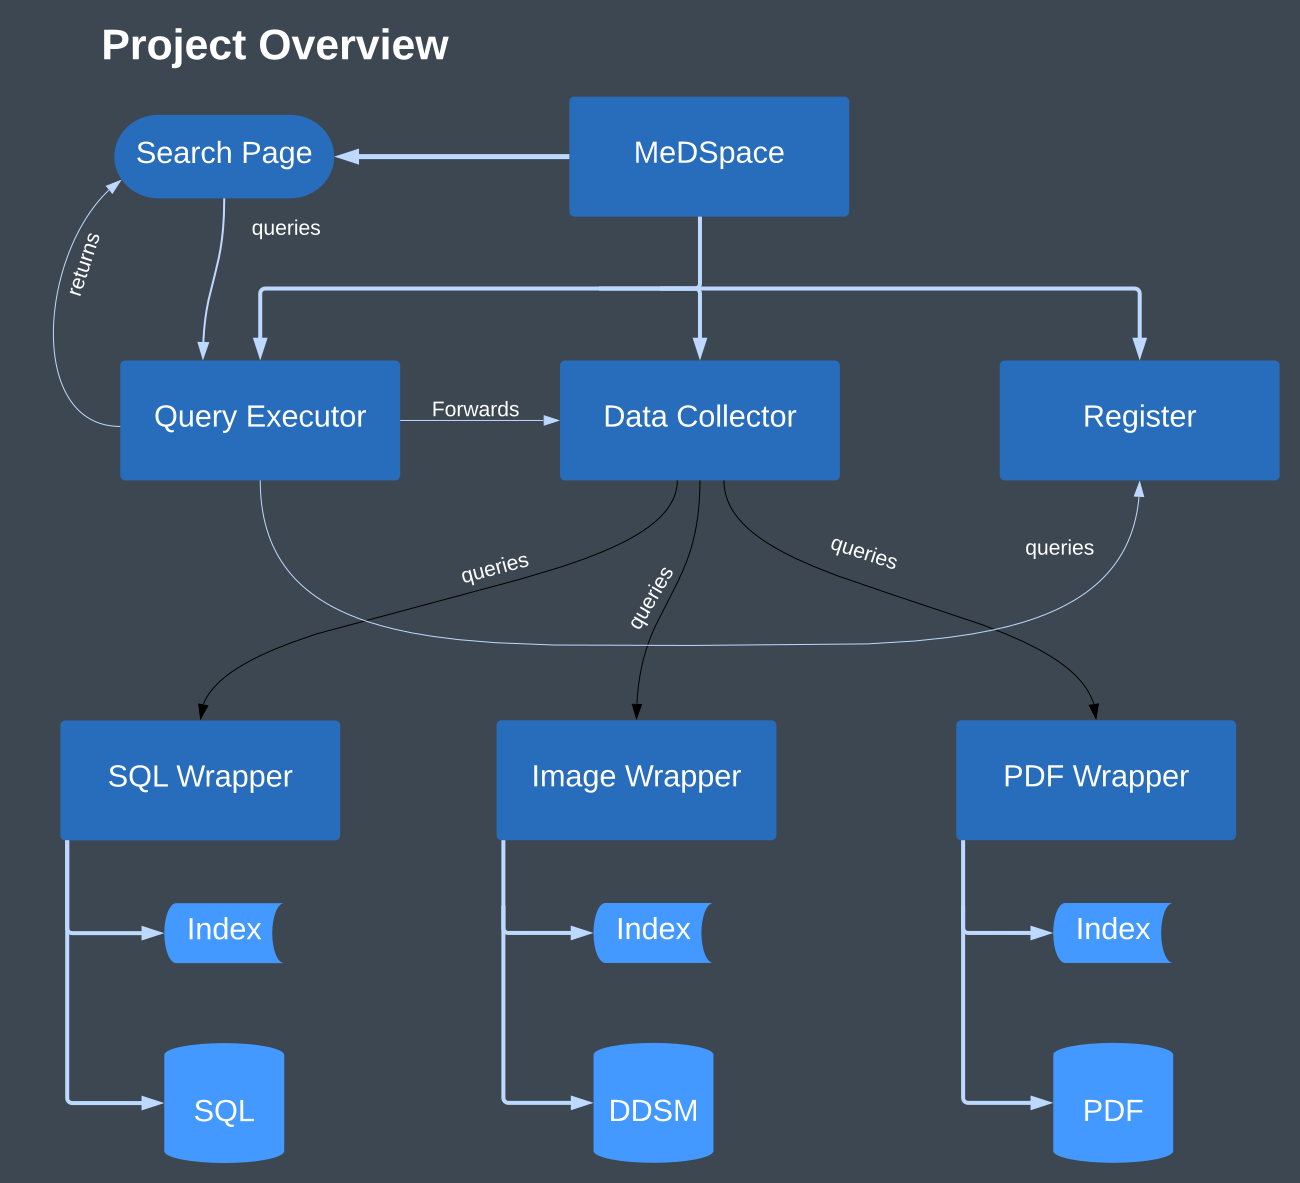
\includegraphics[scale=0.145]{figures/MeDSpace-Overview.png}
	\end{center}
	\caption{MeDSpace Project overview}
	\label{MeDSpaceOverview}
\end{figure} 

The system can roughly be divided into a \emph{wrapper} and a \emph{global MeDSpace} category: The \emph{wrapper} category includes everything from managing the data of a specific datasources (e.g. from a relational database). 
Whereas the \emph{global MeDSpace} category comprises datasource management and services on a global view.  The modules belonging to this category are the \emph{Register}, the \emph{Data Collector}, the \emph{Query Executor}, and the \emph{Search Page}.  

Now, we want to look at the requirements met by MeDSpace. Therefore we look at the purposes of each module of the system.

\section{General} 
MeDSpace uses RDF \cite{w3RDF} as its canonical data model. Although a dataspace system is not restricted to use a specific data model, it simplifies the complexity of data management.
Furthermore RDF is proposed to be used for Linked Data \cite{LinkedData} in the Semantic Web field. Although a different research field, both fields face semantic data-integration.

All wrappers and the register have configuration files. These configuration files use XML, and each configuration file has a corresponding \emph{XML Schema Definition} (XSD)\cite{w3XMLSchema} file, that is used to validate the configuration file. This allowed us to generate automatically Java classes out of the XSD files using \emph{Java Architecture for XML Binding} (JAXB) \cite{JAXB}.


\subsection{Importance of unicode}

A dataspace includes data sources possibly spread around the globe. It is near inferring to support a wide area of different languages. In terms of character sets, it is therefore necessary to use a unicode encoding.
Unicode is a system assigning each character a unique code point and is designed to support the worldwide interchange, processing and display of texts written in different languages\cite{UnicodeStandard}.\newline
There exist several encodings for unicode. The better known are are the UTF and UCS encoding families. In the draft of HTML5 is advised to use UTF-8 for new web pages\cite{HTML5Rec}. 
Thus, to simplify processing we follow the recommendation and use UTF-8 throughout MeDSpace. If a data source doesn't use UTF-8, it is the task of its wrapper to do a proper conversion to UTF-8.

\subsection{Keyword query language convention}
As already previously told, the one service that every wrapper has to implement is the keyword search functionality. In order to search for specific keywords, it is important to define a convention how the keyword search should work, since there are several possibilities. E.g. if a query is posed with two keywords, should a query be created for all results that contains both keywords, or is it enough if one of the keywords is contained? Should boolean operators be allowed (AND, OR, NOT)? 

The design decision is at follows: Rudimentary keyword search functionality suffices and several keyword searches have to be interpreted in an 'AND like' manner by default, i.e. all of the stated keywords have to occur to fulfill the query condition. Additionally the user should be able to use an 'OR' operator instead. This option is provided by the search page.

The reasons are: no complex global query language is necessary that all wrappers have to implement, and this leads to much more flexible implementation decisions. 
We think that it is more likely for a user to achieve results including all stated keywords and not only one of them. So we decided to use the 'AND' operator by default. 
In certain cases the use of the 'OR' operator might be helpful, so we added it, too.
As wrappers can provide as many services as wanted, it is easy to provide a much more powerful keyword search service. So this design decision doesn't restrict the power of a wrapper.


\section{Wrappers}
Each local datasource has its own wrapper. The wrapper is similar to the wrappers used in a mediator-based system, but provides dataspace specific functionality: the wrapper...
\begin{itemize}
	\item manages the data exchange between the datasource and extern MeDSpace services.
	\item provides keyword search functionality (if the data source does not already provide it itself). Therefore it creates an index of the data of the wrapped datasource and maintains it. 	
	\item converts search results from the datasource to the canonical data model.
	\item registers and deregisters the datasource from MeDSpace by communicating with the \emph{Register} module. The wrapper informs the register about the services the datasource and the wrapper provide.
	\item overcomes technical, syntactic and data model heterogeneity. 
\end{itemize}

Thereby the \emph{SQL Wrapper} is responsible for wrapping a relational database containing data created with the \emph{Patient Data Generation Framework} (PDGF) tool created by Schmiedbauer \cite{SchmidbauerBachelorThesis}. The \emph{Image Wrapper} provides access to case files of \emph{Digital Database for Screening Mammography} (DDSM)\cite{DDSM} and the \emph{PDF Wrapper} maintains a set of pdf files that were created specific for this system: the pdf files contain data based on Schmidbauer's test data.

\section{Register}
The Register holds a list of active datasources that can be queried. Therefore it provides functionality so that wrappers can register and deregister a datasource. In order to know what services are provided by each datasource, the register also keeps records of these services. This allows other modules to use services of any datasource.
\section{Query Executor}
The task of the \emph{Query Executor} is to accept a given keyword search query, transform this query to a service call, and instructs the \emph{Data Collector} module to call the keyword search service for each registered datasource. To know which datasources are registered, this module communicates with the \emph{Register} module. After the \emph{Data Collector} has collected the query results of all datasources the \emph{Query Executor} adds the search query to its query cache and returns the collected search result to the caller who requested the \emph{Query Executor}. On the next request the cached query result will be returned without querying the datasources if no 'cache miss' has been occurred.

Note: It is not the task of the \emph{Query Executor} to actually collect the search result from the datasources. That is done by the \emph{Data Collector}. It does only instruct the \emph{Data Collector} to do the collecting.

\section{Data Collector}
The \emph{Data Collector} provides services that allow to query a specific  datasource and store the query result into a specific RDF repository which is maintained by this module. Furthermore the \emph{Data Collector} allows other modules to create and remove a repository that is coupled with a specific search query. This allows the \emph{Query Executor} to merge the search results of all datasources into a seperate RDF repository. Then, again the \emph{Query Executor} is able to delete the repository if the associated and cached query result should be deleted. 

\section{Search Page}
The Search Page represents the \emph{graphical user interface} (GUI) so that a user can easily interact with the MeDSpace system using a common browser. It provides a page for stating and sending keyword searches, allows the user to display the search result in the browser or download it as a file. Furthermore the search page allows the user to inspect the list of the current registered datasources and to delete the query cache.

\chapter{Implementation}
In this chapter we focus on implementation details of the MeDSpace system: 

\begin{itemize}
\item the used technology
\item the implementation structure
\item reasons for using this kind of    
   implementation structure
\item details explained for users and developers to 
   use the system correctly. 
\end{itemize}

\section{Used technologies}

In this section we want to present the technologies used in MeDSpace and explain for each technology the areas of application.

\subsection{Programming language - Java}
MeDSpace is written completely in Java 8. The reason for java are diverse: 
\begin{itemize}
\item its platform independence is very helpful in a heterogeneous environment
\item Not reaching the performance of C++, Java with its JIT compiler has decent performance \cite[p. 425]{TABOADA2013425}. Even though performance isn't the most important, it should not be 
  neglected, as the system potentially has to handle very large data sets
\item last but not least, Java has great library support for Web development
\end{itemize}

Of course, other languages could be used, too, but Java definitively is a good choice.


\subsection{Resource Description Framework}

The \emph{Resource Description Framework} (RDF) \cite{w3RDF} is used as the canonical data model in MeDSpace. Figure \ref{RdfTriple} shows how rdf data is structured. RDF is a graph-based abstract data model. With abstract we mean it is a conceptual data model, so RDF says nothing about serializing data. But there exists plenty serialization formats that can be used to serialize RDF data. A popular RDF serialization format is Turtle \footnote{\url{https://www.w3.org/TR/turtle/}} that is known to be easily human readable.
It facilitates merging data expressed in different schemas, as objects are identified by URIs, and with the help of ontologies semantic data integration can be performed by logical inference. 


\begin{figure}[H]
	\begin{center}
		\includegraphics[scale=0.75]{figures/rdf-graph.pdf}
	\end{center}
	\caption{A predicate connects two nodes (Subject, Object) forming an RDF Triple}
	\label{RdfTriple}
	\footnotemark
\end{figure}
\footnotetext{\url{https://www.w3.org/TR/rdf11-concepts/rdf-graph.svg}}

RDF data consists of resources which are the nodes of the rdf graph, and predicates which are directed edges between the resources. So RDF is a directed graph. 

Resources can be IRIs, literals, and blank nodes. 
Resources with an IRI are identified through its IRI. Two resources with the same IRI are supposed to be equal.
Blank nodes are also called anonymous resources, as they specify the existence of an abstract thing, but it is not identifiable. So blank nodes are always unique.
Literals are used for values like numbers, strings or a date, but aren't identifiable, too.
Predicates are always IRIs and can also be resources. They are also identified by their IRIs.

The idea of RDF is to represent data in form of triple statements that consists of two resources (subject and object in figure \ref{RdfTriple}) and a predicate. The statement 'A has a property B' could be expressed in RDF with two resources, A (the subject) and B (the object) and a predicate with an IRI that should form the 'has' predicate. It should be noted that a subject can be an IRI or a blank node, but not a literal. As a result no statements can be made about a literal.

Listing \ref{listing1} shows an example of how rdf data can look like using Turtle syntax. In line 3 we can see the aforementioned example statement 'A has B'. An interesting property of Turtle is the ability to define prefixes for namespaces, as done at line 1. Prefixes are used to shorten IRIs, thus increasing readability. Thus, the statement in line 3 and the statement in line 5 are equal: in line 3 the fully qualified IRIs are used, whereas in line 5 the 'ex' namespace prefix is used.

Line 7 shows an example of a statement with a literal value.

Line 8 and 9 shows two different ways of blank node usage: In line 8 a so-called 'labeled' blank node is created. This allows a developer to give a blank node same properties by using the labeled like an IRI. A property is stated for this labeled blank node at line 11.
But it should be noted that a blank node is not visible from the outside (i.e. in a SPARQL query).
In line 9 the usage of an 'unlabeled' blank node is illustrated: everything that belongs to the blank node is defined inside the rectangular brackets. \\

\begin{lstlisting}[style=RdfCodeStyle, caption=RDF example data in Turtle syntax, label=listing1]
@prefix \[ex:\] <http://example.org/#>

<http://example.org/#A> 
		<http://example.org/#has> <http://example.org/#B> .

\[ex:\]A \[ex:\]has \[ex:\]B .
\[ex:\]A \[ex:\]hasLiteral 20 .
\[ex:\]A \[ex:\]hasLabeledBlankNode \[_:\]blank .
\[ex:\]A \[ex:\]hasUnlabeledBlankNode [ \[ex:\]hasLiteral 5 ] .

\[_:\]blank \[ex\]:hasLiteral 5 .
\end{lstlisting}


In MeDSpace we used the RDF4J framework (version 2.2.2) \cite{RDF4J} that enabled us to read and write RDF content from within Java. Originally we planned to use Apache Jena \cite{Jena}, but it wasn't possible for us to convert the RDF data into appropriate input and output stream classes without the Jena PipedRDFIterator class \footnote{\url{https://jena.apache.org/documentation/javadoc/arq/org/apache/jena/riot/lang/PipedRDFIterator.html}}, that unfortunately creates a new thread for processing the rdf triples. But that isn't an option for us, as this solution doesn't scale well. 
MeDSpace uses its own interfaces for handling rdf data in order to be independent from any third party framework. Thus it would be relatively easy to support a different rdf framework. To do so, one can implement a custom version of the \emph{de.unipassau.medspace.rdf.RDFProvider} interface. 

\subsection{Apache Lucene}

Apache Lucene is a full-featured text search engine \cite{LuceneCore} at version 6.6.6. In MeDSpace it is used to implement the keyword search functionality and for the search indexes used by the wrappers.

\subsection{Play Framework}

Play is a framework for web development and written in Scala, but it provides Java bindings \cite{Play}. So it is possible to use Play without any complications. In MeDSpace we used Play in its version 2.6.6. We utilized the framework for implementing the REST services and for the GUI. 

Play has its own default folder structure. In order to understand how the modules are structured, it is necessary to have at least a rough understanding of it:

\begin{itemize}
\item \textbf{app} In this folder all the source code is stored. This includes also html templates that are used to generate dynamic html pages. These templates have to be stored in the subfolder  \emph{views}. The same applies to controllers which have to be stored inside the \emph{controllers} subpackage.

\item \textbf{conf} Contains configuration files. The  file \emph{application.conf} is used to configure the Play framework (e.g. the port number for the http server should run on). The \emph{logback.xml} file is the configuration file for the logging backend logback \footnote{\url{https://logback.qos.ch/}} and the file \emph{routes} contains the definition of relative URL to java method mappings. This is used to define on which URL a service is located. As some modules call services by its URL name, the URLs routes shouldn't be modified carelessly. For example, if you change the relative URL for registering a datasource, all wrappers have to be updated to use the new URL.

\item \textbf{public} Resource folder for the http server. Here is stored static content that should be transferred to a client, like javascript files or css files.

\item \textbf{project} Contains additional build configurations. E.g. we used the sbt-sass plugin to compile sass to a css file. 
\end{itemize} 

Play needs the Simple Build Tool \cite{SBT}(SBT). As a consequence we had to use SBT, too. Thus we used SBT as build tool for the whole project. If you just want to run MeDSpace, SBT is not required, but if you want to compile it you must have installed it at least on version 0.13.15 . 

The play framework supports dependency injection powered by Google's Guice \footnote{\url{https://github.com/google/guice}}. This way it is possible to inject dependencies by defining a special class that is instantiated by Play on startup. The definition of this class is done in the \emph{application.conf} file by assigning the property \emph{play.modules.enabled}. In MeDSpace this functionality is used to inject global class instances, e.g. for providing access to the configuration files or access to rdf processing methods.

\subsection{JAXB}

With the Java Architecture for XML Binding \cite{JAXB} (JAXB) we mapped the XML configuration files to auto-generated Java classes. This simplified the configuration reading, reduced programming faults, and enabled us to do changes faster. If you want to generate the java classes by yourself, you have to look at the subfolder \emph{jaxb-generation} of your target module (e.g. sql wrapper). There you'll find batch and shell scripts you just have to execute. The only requirement is that the \emph{xjc} binary is findable through the environment variable of your operating system. This should be the case if you properly have installed the JDK.

All xjc generation commands are structured as follows:

\begin{codebox}
	\textbf{xjc} \textbf{-b} 'binding-file' \textbf{-p} 'target-package' \textbf{-d} 'output-directory' \textbf{-extension} 'target-xsd-file'
\end{codebox}

The \emph{binding-file} is used to customize the generated java classes, e.g. the class can be assigned a different class name, \emph{output-directory} specifies the directory where the generated java classes should be saved to, and \emph{target-xsd-file} is the xsd file to use. The xsd file is the specification how the XML configuration should look like and therefore from the xsd file the java classes can be derived from.

In listing \ref{jaxbExample} you can see an extract of \emph{medspace-d2rmap-binding.xml}, where a complex type \emph{Bridge} from the \emph{Medspace\_D2Rmap.xsd} xsd file is mapped to a class called \emph{BridgeParsing}:

\begin{lstlisting}[style=RdfCodeStyle, caption=JAXB binding example, label=jaxbExample]
<jxb:bindings 
    xmlns:xsd="http://www.w3.org/2001/XMLSchema"
    xmlns:jxb="http://java.sun.com/xml/ns/jaxb"
    version="2.1">

    <jxb:bindings schemaLocation="Medspace_D2Rmap.xsd">
		<jxb:bindings node="//xsd:complexType[@name='Bridge']">
			<jxb:class name="BridgeParsing"/>
		</jxb:bindings>
    </jxb:bindings>
</jxb:bindings>
\end{lstlisting}

\section{Wrappers - General}

This section targets to present implementation details that is used by all wrapper implementations.

Each wrapper has a \emph{general-wrapper-config.xml} configuration file that is located in the \emph{medspace} subfolder of the respective wrapper. This configuration file has to follow a specific structure that is defined in \emph{medspace-wrapper-config-specification.xsd}. This XSD file is used to validate the general wrapper configuration file. The XSD file can be found as a resource file in the \emph{commons} package: \\
\emph{\{medspace-root-folder\}/commons/src/main/resources}

The following items can be configured through this configuration file:
\begin{itemize}
\item \textbf{Services}: Specifies which services the wrapper supports. The name of the service is thereby the relative path for calling the service. MeDSpace translate this then to an absolute URL by using the wrapper host address, the url would be \emph{\{wrapper-address\}/\{service-name\}}. 

Example: if the wrapper address is \emph{http://localhost:9300} and the service  name is \emph{keyword-search}, then the resulting absolute URL would be: \emph{http://localhost:9300/keyword-search}. 

It should be noted that MeDSpace expects the services in \textbf{lower case}. So you shouldn't define service URLs that use upper case characters, as URLs are \textbf{case sensitive}.
Furthermore is expected from every wrapper to support the keyword-search service. So it is not explicitly necessary to state it in the configuration file.

\item \textbf{IndexDirectoy}: The directory where index data should be stored. If the directory already contains indexed data, the wrapper will use it.

\item \textbf{Namespaces}: Defines prefixes for rdf namespaces. 

\item \textbf{OutputFormat}: Specifies the RDF syntax, the wrapper should use.

\item \textbf{RegisterUrl}: The URL to the register.

\item \textbf{ConnectToRegister}: Specifies whether the wrapper should register itself on startup. This is primarily for testing and debugging.
\end{itemize}

\subsection{Indexing}

On startup the wrapper tries to fetch and index the data from the datasource for the keyword search functionality. If the index exists already (e.g. from a previous run), the wrapper won't reindex the data. But the wrapper provides a service for reindexing the data on runtime. The service can be found at \emph{/reindex}, uses no argument and http \emph{GET}.

\subsection{Keyword search service}

Each wrapper supports keyword search functionality. The corresponding service can be found under 
\textbf{/keyword-search}, uses http GET, and needs the following arguments:
\begin{itemize}
\item \textbf{keywords}: A list of keywords to search for. The keywords have to be separated by spaces or commas.
\item \textbf{useOr}: Specifies if the OR operator should be used instead of AND. This argument is optional. Its default value is \emph{false}.
\item \textbf{attach}: Specifies whether the result should be interpreted as a file attachment. This opetion is only relevant for browser. This argument is optional. Its default value is \emph{false}.
\end{itemize}


\section{SQL Wrapper}

In this section we will talk about implementation details of the SQL wrapper. 
The task of the SQL Wrapper is to convert the relational data into RDF and providing a keyword search functionality, as SQL databases don't provide this kind of  functionality.
We used a MySQL datasource, but as several other relational databse vendors exist, one additional design goal was to produce a wrapper that can be used with any other database that uses SQL for querying. That will considerably reduce prospective maintenance work.
Thus, a SQL wrapper was implemented, that doesn't use any vendor specific features.

Before discussing how to perform the conversion from SQL to RDF, we want to look at the proper setup of the MySQL database.



\subsection{Setting up a MySQL data source}

To setup a MySQL datasource get a recent stable MySQL community server\footnote{\url{https://www.mysql.de/downloads/}} 
and install it for your target platform. Additionally you will need the Connector/J components, the official JDBC driver for MySQL. 

At time of writing the most recent stable versions are the community server 5.7.17 and the Connector/J 5.1.41. These versions are used for the thesis project and all following commands are related on them. If you're using 
different versions, assure that the instructions are adapted properly. As a detailed installation instruction for all supported platforms would break the mold, the reader is encouraged to consult the official 
manual\footnote{\url{https://dev.mysql.com/doc/}}. 
Assure that the MySQL binary folder is integrated into your class path, so that you can access it globally in a shell/command line. Although not necessary, it is recommended for security reasons 
to set a password for the root user\footnote{\url{https://dev.mysql.com/doc/refman/5.7/en/default-privileges.html} , \url{https://dev.mysql.com/doc/refman/5.7/en/resetting-permissions.html}}. 
After installing the server, do postinstallation setup and testing\footnote{\url{https://dev.mysql.com/doc/refman/5.7/en/postinstallation.html}}. 

To support UTF-8 set in your my.cnf 

\begin{codebox}
	default-character-set = utf8
\end{codebox}

in the mysql section and

\begin{codebox}
	character-set-server=utf8\newline
	collation\-server=utf8\_general\_ci
\end{codebox}

in the mysqld section. Then restart the mysqld daemon. In the following it is assumed that you have a running MySQL server now that can be accessed via shell/command line. Before you connect to the MySQL server, you should assure that the application you use for connecting is using UTF-8 for user input and sending statements. So, validate that your shell/command line is using UTF-8. E.g. on windows system (before Windows 10) the command line isn't using UTF-8 by default
\footnote{To set the encoding to UTF-8 on the windows command line change the active code page to 65001 and set 'Lucida Console' as the displaying font. In contrast to the font the code page is only active for the current console session. But you can automate this command with a AutoRun setting. For more information see \url{https://blogs.msdn.microsoft.com/oldnewthing/20071121-00/?p=24433}}.  
Now try to connect to the database as the user root:

\begin{codebox}
	mysql -u root -p 
\end{codebox}

If you've done all right, you should be connected to the database after entering and confirming the password that you've previously stated for the user root.

The next step is to validate that UTF-8 is indeed continuously used. Execute:

\begin{codebox}
	SHOW VARIABLES LIKE 'char\%';
\end{codebox}

and check that the variables \emph{character\_set\_client}, \emph{character\_set\_connection}, \emph{character\_set\_database}, \emph{character\_set\_results}, \emph{character\_set\_server} and \emph{character\_set\_system} are all set to utf8.
Basically these variables are used to interpret and write data consistently in UTF-8. More information about the stated variables can be found on the manual
\footnote{\url{https://dev.mysql.com/doc/refman/5.7/en/server-system-variables.html\#sysvar_character_set_client}}.

The next step is to initialize the data source with a database and some content. Further we need a user which is used by the wrapper to communicate with the data source. The wrapper needs no writing rights and indeed we don't want it to change the data, so following the security rule 'As few rights as possible' we grant this user only reading rights for fetching data. The commands for initializing the data source and creating a read-user are in the file \textbf{init\_mysql.sql} which is located in the appendix data in the folder \textbf{implementation/SQL/mysql}.

To execute commands from a file execute while logged in as the root user:

\begin{codebox}
	SOURCE \emph{path\_to\_sql\_file};
\end{codebox}

where \emph{path\_to\_sql\_file} is the full (absolute or relative) path to the sql file.
By default the created database will be named \textbf{medspace} and the read-user will be called \textbf{medspace\_client}. If you want to edit the init.sql file, beware that the file is encoded in UTF-8. As we instructed mysql to use UTF-8 in every case, this encoding is required. Assure that your file editor saves the file in that encoding, too. Otherwise, it could come to conversion errors.


\subsection{D2RMap}

In this sub section we want to look at the conversion from SQL to RDF. To do this the wrapper implements a specialized version of the D2rMap language. D2rMap was designed by Chris Bizer and is  a declarative language to describe mappings between relational databases schemata and OWL/RDFS ontologies\cite{D2rMap_aDatabaseToRdfMappingLanguage}.

D2rMap is a general purpose language to export any SQL data to RDF. To better suit the needs for a dataspace wrapper the language was changed. The custom language is called \emph{MeDSpace D2RMap} and its language specification is defined in \emph{MeDSpace\_D2RMap\_Language\_Specification.pdf} which is shipped with MeDSpace. But in general it is very similar to the original D2rMap.\\

The mapping is done as follows: At first the user specifies mappings in a config file. 
The mapping process is visualized in figure \ref{D2rMappingProcessFigure}.

\begin{figure}[H]
	\begin{center}
		\includegraphics[width=0.75\textwidth]{figures/MappingProcess.png}
	\end{center}
	\caption{The D2r mapping process \cite{D2rMap_aDatabaseToRdfMappingLanguage}}
	\label{D2rMappingProcessFigure}
\end{figure}

Each mapping is used to create RDF instances of a certain type. The mapping contains a SQL query that represents all the necessary data for creating the instances. Furthermore, in the mapping are columns specified that are used to create unique IDs for the created RDF instances.
The next step is to fetch the SQL data and group the record set according to the fore mentioned columns. Now, each row of the grouped record set represents a RDF instance, so the instances can be created by proceeding all rows. The last step is the creation of the property statements of the RDF instances. Important to note is the seperation of the last two steps. As all RDF instances exists before the properties are created, it is possible to reference other RDF instances (from the same mapping or another).

An example of a mapping between a SQL query and RDF data definition is showed in listing \ref{D2RMapMappingExample}

\begin{lstlisting}[style=RdfCodeStyle, caption=Example of a MeDSpace D2rMap mapping, label=D2RMapMappingExample]
<d2r:ClassMap
			type="test:doctor"
			sql="SELECT * FROM doctor"
			resourceIdPattern="@@id@@"
			id="doctor">

		<d2r:DataTypePropertyBridge property="doctor:id" pattern="@@id@@" dataType="xsd:integer"/>
		<d2r:DataTypePropertyBridge property="doctor:firstname" pattern="@@firstname@@" dataType="xsd:string"/>
		<d2r:DataTypePropertyBridge property="doctor:lastname" pattern="@@lastname@@" dataType="xsd:string"/>
		<d2r:ObjectPropertyBridge property="doctor:hospital" referredClass="hospital" referredColumns="doctor.hospital"/>

		<d2r:MetaData>person doctor clinician</d2r:MetaData>
	</d2r:ClassMap>

\end{lstlisting}

In the listing relational data for doctors working in a hospital is mapped to RDF. The rdf type is specified in line \textbf{3}, and in line \textbf{4} the SQL query is specified that should be executed to collect the data. 

The \emph{DataTypePropertyBridge} tag defines rdf statements that have a literal value (e.g. the name of the doctor). 
With \emph{ObjectPropertyBridge} rdf statements to other class mappings can be defined. In the above example the doctor class map references a hospital class map that is not shown in the listing. 

Names that are enclosed by two '@@' specify a value of a column. E.g. with '@@firstname@@' is meant the value of the column \emph{firstname} which is part of the sql query 'SELECT * FROM doctor'.

With the \emph{MetaData} one can specify tags for the rdf data. This is useful for the keyword search in MeDSpace, as additional domain knowledge can be stated that should be searchable. That way it is possible to get doctor rdf data in the search result if you search for 'person' or 'clinician'. 

\subsection{Keyword search}

After discussing the SQL to RDF mapping we now look at the keyword search, now:
Mainly there are two possibilities to implement a keyword search functionality:
\begin{itemize}
	\item {Construct a keyword search query in SQL and let the database answer the query}
	
	\item {Use a keyword search engine that answers the query based on an external index}
\end{itemize}

At first glance the first option sounds obviously simple, but after implementing it showed several disadvantages: SQL is not designed to provide search functionality based on keywords. SQL uses the \textbf{\emph{LIKE}} operator for pattern matching. But in order to do a Full-text search the SQL Query executor cannot use any index resulting in poor query answer performance. Another problem of \emph{LIKE} is that there is no way to define searching only whole words and not just sub word matching. Whole word matching is very important, as e.g. a user searching for data about male patients should not get also data about female patients.
As a result the \emph{LIKE} operator is not suitable for a proper keyword search service as expected to be provided by a dataspace wrapper. Several SQL database vendors often provide own solutions for Full-Text search queries. But these solutions often have restrictions, as e.g. only column fields having the datatype \emph{TEXT} (on MySQL), and the fields have to be specified as fulltext fields (in their creation or through an update operation) so that the SQL engine is able to create an index for it (at MySQL databases at least).\\
A Wrapper could use vendor specific services but obviously that would exclude other SQL database vendors.

The second option doesn't rise the aforementioned issues of option one. For the Wrapper a keyword searcher was implemented using the fulltext search engine Apache Lucene. The advantage of using Lucene is it's high-performance and scaling of keyword searches over large data sets. Additionally it allows a fine granular configuration about the query construction and sorts automatically the query result by relevance (so called query result ranking). \\
The major disadvantage of using lucene is that the SQL data have to be extracted and indexed outside the database. If the data changes or rows are added resp. deleted, the index has to be updated accordingly. The update process can be very complex, as not only new data has to be indexed resp. existing data has to be removed, but also data that references the deleted, or new data that depends on it.\\
A simpler but obviously slower solution is to reindex the whole data set. Reindexing the whole data set is only advised if updates occur not very often, or if acceptably, when the wrapper updates the index not instantly and thus provides potentially outdated data.

The decision which method is more suitable depends primarily on the use case and the domain. As the project is designed to be used as a test suite for medical datasources and medical science, it is acceptable if the data is outdated a bit to some degree and will be updated at every database change. So, changes on the datasource haven't to be updated in near-realtime.

Then one of the design goals for this project was to design a SQL wrapper that can be used with arbitrary vendors. As a result, vendor specific services are not an option.

All things considered the preferred method for the keyword search functionality clearly is Apache Lucene Core, as the advantages by far outweigh outweigh its disadvantages. Thus, a full functional keyword searcher was implemented powered by Lucene.


\section{Image Wrapper}
 
In this section details about the implementation of the image wrapper are presented. 
At first we want to look at the data the image wrapper is managing. Then we will discuss how the data is indexed, mapped, and converted to RDF. Finally we present the multimedia file download service that allows others to access the source files of DDSM cases.

\subsection{DDSM}

The data managed by the image wrapper are DDSM case file that are publicly available\footnote{\url{http://marathon.csee.usf.edu/Mammography/Database.html}}.
DDSM is a resource for mammographic image analysis and it contains data about approximately 2500 cases \cite{DDSM}. As one case needs relative much disk space, we decided to use only a subset of 50 cases that take altogether 3.7 GB.

In the following we will touch upon the content of a case, but for more details, please consult the specification of a DDSM case \cite{DDSM_CASE_SPEC}. 

For each study a case contains two LJPEG images for each breast (so 4 images in total) and related patient information. LJPEG is a very old image format that nowadays isn’t used very often anymore. In fact, we didn't found a tool, that could display it. Thus, we decided to convert the images to PNG. Hence, we used Sharma's \emph{DDSMUtility} \cite{DDSM_UTILITY}.

A case also contains a 16\_PGM image that is an overview of the whole case. But the 16\_PGM image is not really needed and as 16\_PGM is a really old image format, we didn't used it.

Each case has a ICS file that holds general information about the case. It also specifies if a so-called overlay is defined for each breast image. 

Overlay files are used to specify found abnormalities in the breast images. An overlay file contains the number of found abnormalities, the type of each abnormality, and defines outline boundaries which specify where the abnormality can be found in the source image.

\subsection{RDF conversion}

The data for each DDSM case is collected and useful data is extracted to create java objects from it. We created java classes for the ics file, overlay file, abnormality, and the lesion types, calcification and mass. The content of each java object, that is created using the aforementioned method, is indexed and stored locally. 

When a keyword search query is executed, the searching module queries the indexed documents. Each document is assigned to a specific java class in order to know that a document represents an ICS file, an overlay file, etc. .  

We defined for each type a RDF mapping that is specified in the configuration file \emph{medspace-ddsm-mapping.xml}. The configuration file has a specification file \emph{medspace-ddsm-mapping-specification.xsd}, so that the mapping types can be auto-generated using JAXB.

With the mapping configuration it is possible to generate RDF data from each document.

\subsection{File downloading service}

For the exported rdf types \emph{IcsFile} and \emph{Overlay}, which represent an ics file resp. overlay file of a DDSM case, we defined statements that point to a URL location of the source file. We decided to implement a service on the image wrapper that allows others to download these image files. 

In listing \ref{FileDonwloadResultExample} you can see an example of created RDF data for a breast image. The highlighted URL specifies the source image. In this example the image wrapper is running at localhost on port 9300, and as stated before, by following the link (e.g. in the browser) it would be possible to download the source image.

\begin{lstlisting}[style=RdfCodeStyle, caption=image RDF conversion example, label=FileDonwloadResultExample]
<http://www.medspace.com/images/ddsm/image#cancers/cancer_01/case0001/C_0001_1.LEFT_CC.png>
image:source \["http://localhost:9300/get-file?relativePath=cancers/cancer_01/case0001/C_0001_1.LEFT_CC.png"\]^^xsd:anyURI .
\end{lstlisting}



\section{PDF Wrapper}
In this section details about the implementation of the PDF wrapper are presented.
At first we look at what data is managed by this wrapper. Then we take a closer look at how the data is indexed, mapped, and converted to RDF. Finally we present the multimedia file download service, that allows others to access the pdf files.

\subsection{PDF Data}

Actually it was planned to use existing PDF files, but we didn't found suitable PDF files that are publicly available and contain healthcare data. As a result, we generated our own PDF files. For this we used again Schmiedbauer's data set and wrote a little PDF generation program that establishes a JDBC connection to the MySQL database and fetches some data. From that data we created PDF files. For the PDF generation we used the framework Apache PDFBox \cite{PDFBox}.  

\subsection{RDF conversion}

On startup the PDF wrapper extracts the content from the pdf files and indexes it. This way it is possible to do a full-text search over all pdf files. 

The mapping to RDF is straight forward: Each pdf file is mapped to a rdf type called 'PdfFile'. The specification of this type is done in the file \emph{medspace-pdf-wrapper-config-specification.xsd} which is used to create auto-generated java classes with JAXB. Also it is used to validate the mapping configuration file. The definition of the mapping is done in the corresponding configuration file \emph{medspace-pdf-wrapper-config.xml}. Listing \ref{PDFWrapperMappingConfig} shows an extract of the configuration file:

\begin{lstlisting}[style=RdfCodeStyle, caption=Extract of the pdf wrapper configuration, label=PDFWrapperMappingConfig]
<pdf:PdfRootDirectory>./_work/pdfFiles/</pdf:PdfRootDirectory>
<pdf:PdfFile rdfType="http://www.medspace.com/pdf/pdf_file" classId="pdfFile">
	<rdf-mapping:metaData>pdf file</rdf-mapping:metaData>
    <pdf:source propertyType="pdf_file:source" dataType="xsd:string"/>
</pdf:PdfFile>
\end{lstlisting}

In line \textbf{1} the directory is specified, where all pdf files are located.
Starting from line \textbf{2} is the definition of the RDF type \emph{PdfFile} which contains the source file location and (optional) meta data tags (as the other wrappers use it).

\subsection{File downloading service}

This service works similar like the one of the image wrapper: every PDF file that is mapped to RDF is assigned a download link so that it can be downloaded from external programs.

Every pdf file gets assigned an ID so that the downloading service can distinguish and locate them. The ID thereby is the file path in relation to the pdf file root directory that is specified in the configuration file.

\section{Global MeDSpace}

In this section implementation details of the global MeDSpace application (\emph{Query Executor}, \emph{Data Collector}, \emph{Register}) are presented.


\subsection{Query Caching}
In this passage details about the implementation of the query caching are explained, a functionality that is implemented in the \emph{Query Executor} module.

For each keyword search query we created unique strings in order to avoid caching duplicates.
The algorithm works as follows: the keywords are transformed to lower case, trimmed, lexically sorted, and finally duplicates are deleted.
For actually caching the query, we used EHCache \cite{EHCache}. 
It should be noted that only the queries itself are cached by EHCache. The result of the query is stored by the \emph{Data Collector} using a \emph{NativeStore}\footnote{\url{http://docs.rdf4j.org/javadoc/2.2/org/eclipse/rdf4j/sail/nativerdf/NativeStore.html}} from the RDF4J framework.

\subsection{Datasource storing}
In this section details about the implementation of the \emph{Register} module are presented.

When the register is shutting down it saves all registered datasources into a local file \emph{datasources.json} in the current working directory. The datasources are serialized to JSON in this file. If MeDSpace finds the aforementioned file, it will auto-register them on startup without contacting the respective datasources.

\subsection{IO-Error policy}

If a datasource doesn't respond anymore, e.g. the network is overloaded or the wrapper doesn't derigester itself for any reason every try to call it's services would inevitable result in a lot of io-errors, slowing down query query answering. Therefore we implemented an io-error policy that works as follows: for every registered datasource a counter for the happened io-errors is hold. Whenever an io-error occurs the counter gets increased. Should the counter exceed a specified limit, the datasource gets deregistered automatically. The default value of the io-error limit is 5, but this can be configured in the \emph{medspace-config.xml} from the \emph{medspace} project.

\section{GUI}
In this section is explained how the GUI of MeDSpace was created.

For dynamic (html) page creation we used Play's template engine \emph{Twirl} \footnote{\url{https://github.com/playframework/twirl}}. The templates are normal text files that are enriched by Scala code \cite{PlayJavaTemplates}.

For styling the html content, we used SASS, an extension of CSS that is used to generate CSS files \cite{SASS}. In order to auto-compile the SASS files we've used the \emph{sbt-sassify} plugin \footnote{\url{https://github.com/irundaia/sbt-sassify}}. 

The look of the search page is illustrated in figure \ref{MeDSpaceSearchPage}:

\begin{figure}[H]
	\begin{center}
		\includegraphics[width=1\textwidth]{figures/MeDSpace-GUI-Search-Main.png}
	\end{center}
	\caption{MeDSpace search page}
	\label{MeDSpaceSearchPage}
\end{figure}

The search page contains a blue header with the writing 'MeDSpace - Testsuite for Medical Information'. Then the navigation menu follows which contains buttons to navigate to the search and datasources page. For each button exists a tooltip describing the respective page. An example of this tooltips is illustrated in figure \ref{MeDSpaceDataTooltip}. 

In the page body is an input field allowing a user to state a keyword search query. The user can state if he wishes to use the OR operator instead of the AND operator, and he can state whether he wants the rdf query result to be returned as a file. Both options can be activated by using the check boxes under the text input field. With the \emph{Search} button the query gets executed.

\begin{figure}[H]
	\begin{center}
		\includegraphics[width=0.7\textwidth]{figures/MeDSpace-GUI-Tooltip.png}
	\end{center}
	\caption{Tooltip of a navigation button}
	\label{MeDSpaceDataTooltip}
\end{figure}


The \emph{Data Sources} page lists all registered datasources, as illustrated in figure \ref{MeDSpaceDataSourcePage}: 

\begin{figure}[H]
	\begin{center}
		\includegraphics[width=1\textwidth]{figures/MeDSpace-GUI-Datasources.png}
	\end{center}
	\caption{Data Sources page}
	\label{MeDSpaceDataSourcePage}
\end{figure}

\textcolor{red}{TODO: Better image}

For each datasource is listed its URL, a description of it, what services it provides, when it registered itself, and how much io errors occurred since its registration.